% Options for packages loaded elsewhere
\PassOptionsToPackage{unicode}{hyperref}
\PassOptionsToPackage{hyphens}{url}
\PassOptionsToPackage{dvipsnames,svgnames,x11names}{xcolor}
%
\documentclass[
  super,
  preprint,
  3p,
  twocolumn]{elsarticle}

\usepackage{amsmath,amssymb}
\usepackage{iftex}
\ifPDFTeX
  \usepackage[T1]{fontenc}
  \usepackage[utf8]{inputenc}
  \usepackage{textcomp} % provide euro and other symbols
\else % if luatex or xetex
  \usepackage{unicode-math}
  \defaultfontfeatures{Scale=MatchLowercase}
  \defaultfontfeatures[\rmfamily]{Ligatures=TeX,Scale=1}
\fi
\usepackage{lmodern}
\ifPDFTeX\else  
    % xetex/luatex font selection
\fi
% Use upquote if available, for straight quotes in verbatim environments
\IfFileExists{upquote.sty}{\usepackage{upquote}}{}
\IfFileExists{microtype.sty}{% use microtype if available
  \usepackage[]{microtype}
  \UseMicrotypeSet[protrusion]{basicmath} % disable protrusion for tt fonts
}{}
\makeatletter
\@ifundefined{KOMAClassName}{% if non-KOMA class
  \IfFileExists{parskip.sty}{%
    \usepackage{parskip}
  }{% else
    \setlength{\parindent}{0pt}
    \setlength{\parskip}{6pt plus 2pt minus 1pt}}
}{% if KOMA class
  \KOMAoptions{parskip=half}}
\makeatother
\usepackage{xcolor}
\setlength{\emergencystretch}{3em} % prevent overfull lines
\setcounter{secnumdepth}{5}
% Make \paragraph and \subparagraph free-standing
\ifx\paragraph\undefined\else
  \let\oldparagraph\paragraph
  \renewcommand{\paragraph}[1]{\oldparagraph{#1}\mbox{}}
\fi
\ifx\subparagraph\undefined\else
  \let\oldsubparagraph\subparagraph
  \renewcommand{\subparagraph}[1]{\oldsubparagraph{#1}\mbox{}}
\fi


\providecommand{\tightlist}{%
  \setlength{\itemsep}{0pt}\setlength{\parskip}{0pt}}\usepackage{longtable,booktabs,array}
\usepackage{calc} % for calculating minipage widths
% Correct order of tables after \paragraph or \subparagraph
\usepackage{etoolbox}
\makeatletter
\patchcmd\longtable{\par}{\if@noskipsec\mbox{}\fi\par}{}{}
\makeatother
% Allow footnotes in longtable head/foot
\IfFileExists{footnotehyper.sty}{\usepackage{footnotehyper}}{\usepackage{footnote}}
\makesavenoteenv{longtable}
\usepackage{graphicx}
\makeatletter
\def\maxwidth{\ifdim\Gin@nat@width>\linewidth\linewidth\else\Gin@nat@width\fi}
\def\maxheight{\ifdim\Gin@nat@height>\textheight\textheight\else\Gin@nat@height\fi}
\makeatother
% Scale images if necessary, so that they will not overflow the page
% margins by default, and it is still possible to overwrite the defaults
% using explicit options in \includegraphics[width, height, ...]{}
\setkeys{Gin}{width=\maxwidth,height=\maxheight,keepaspectratio}
% Set default figure placement to htbp
\makeatletter
\def\fps@figure{htbp}
\makeatother

\makeatletter
\makeatother
\makeatletter
\makeatother
\makeatletter
\@ifpackageloaded{caption}{}{\usepackage{caption}}
\AtBeginDocument{%
\ifdefined\contentsname
  \renewcommand*\contentsname{Table of contents}
\else
  \newcommand\contentsname{Table of contents}
\fi
\ifdefined\listfigurename
  \renewcommand*\listfigurename{List of Figures}
\else
  \newcommand\listfigurename{List of Figures}
\fi
\ifdefined\listtablename
  \renewcommand*\listtablename{List of Tables}
\else
  \newcommand\listtablename{List of Tables}
\fi
\ifdefined\figurename
  \renewcommand*\figurename{Figure}
\else
  \newcommand\figurename{Figure}
\fi
\ifdefined\tablename
  \renewcommand*\tablename{Table}
\else
  \newcommand\tablename{Table}
\fi
}
\@ifpackageloaded{float}{}{\usepackage{float}}
\floatstyle{ruled}
\@ifundefined{c@chapter}{\newfloat{codelisting}{h}{lop}}{\newfloat{codelisting}{h}{lop}[chapter]}
\floatname{codelisting}{Listing}
\newcommand*\listoflistings{\listof{codelisting}{List of Listings}}
\makeatother
\makeatletter
\@ifpackageloaded{caption}{}{\usepackage{caption}}
\@ifpackageloaded{subcaption}{}{\usepackage{subcaption}}
\makeatother
\makeatletter
\@ifpackageloaded{tcolorbox}{}{\usepackage[skins,breakable]{tcolorbox}}
\makeatother
\makeatletter
\@ifundefined{shadecolor}{\definecolor{shadecolor}{rgb}{.97, .97, .97}}
\makeatother
\makeatletter
\makeatother
\makeatletter
\makeatother
\usepackage{float}
\makeatletter
\let\oldlt\longtable
\let\endoldlt\endlongtable
\def\longtable{\@ifnextchar[\longtable@i \longtable@ii}
\def\longtable@i[#1]{\begin{figure}[H]
\onecolumn
\begin{minipage}{0.5\textwidth}
\oldlt[#1]
}
\def\longtable@ii{\begin{figure}[H]
\onecolumn
\begin{minipage}{0.5\textwidth}
\oldlt
}
\def\endlongtable{\endoldlt
\end{minipage}
\twocolumn
\end{figure}}
\makeatother
\journal{IEEE VizCorner}
\ifLuaTeX
  \usepackage{selnolig}  % disable illegal ligatures
\fi
\usepackage[]{natbib}
\bibliographystyle{elsarticle-num}
\IfFileExists{bookmark.sty}{\usepackage{bookmark}}{\usepackage{hyperref}}
\IfFileExists{xurl.sty}{\usepackage{xurl}}{} % add URL line breaks if available
\urlstyle{same} % disable monospaced font for URLs
\hypersetup{
  pdftitle={ITS\_LIVE: A Cloud-Native Approach to Monitoring Glaciers from Space},
  pdfauthor={Luis A. López; Alex S. Gardner; Chad A. Greene; Mark Fahnestock; Joseph H. Kennedy; Maria Liukis; Theodore A Scambos; Jacob R. Fahnestock},
  pdfkeywords={glaciology, climate change, big data, cloud computing},
  colorlinks=true,
  linkcolor={blue},
  filecolor={Maroon},
  citecolor={Blue},
  urlcolor={Blue},
  pdfcreator={LaTeX via pandoc}}

\setlength{\parindent}{6pt}
\begin{document}

\begin{frontmatter}
\title{ITS\_LIVE: A Cloud-Native Approach to Monitoring Glaciers from
Space}
\author[1]{Luis A. López%
%
}
 \ead{luis.lopezespinosa@colorado.edu} 
\author[2]{Alex S. Gardner%
%
}
 \ead{alex.s.gardner@jpl.nasa.gov} 
\author[2]{Chad A. Greene%
%
}
 \ead{chad.a.greene@jpl.nasa.gov} 
\author[3]{Mark Fahnestock%
%
}
 \ead{mfahnestock@alaska.edu} 
\author[3]{Joseph H. Kennedy%
%
}
 \ead{jhkennedy@alaska.edu} 
\author[2]{Maria Liukis%
%
}
 \ead{maria.liukis@jpl.nasa.gov} 
\author[5]{Theodore A Scambos%
%
}
 \ead{tascambos@Colorado.EDU} 
\author[6]{Jacob R. Fahnestock%
%
}
 \ead{jrfz31@gmail.com} 

\affiliation[1]{organization={NSIDC, University of Colorado
Boulder},,postcodesep={}}
\affiliation[2]{organization={NASA, Jet Propulsion
Laboratory},,postcodesep={}}
\affiliation[3]{organization={UAF, Geophysical
Institute},,postcodesep={}}
\affiliation[4]{organization={UAF, Alaska Satellite
Facility},,postcodesep={}}
\affiliation[5]{organization={CIRES, Earth Science and Observation
Center},,postcodesep={}}
\affiliation[6]{organization={Wentworth Institute of
Technology},,postcodesep={}}

\cortext[cor1]{Corresponding author}








        
\begin{abstract}
NASA's ITS\_LIVE project delivers near-real-time information on global
glacier dynamics and provides historical context for climate change with
a record of how every glacier in the world has evolved over decades of
satellite observation. To handle petabytes of data in the satellite
archives and a constant influx of new observations, ITS\_LIVE has
adopted a modern cloud-native approach that is scalable, highly
performant, user friendly, and embraces transparent and collaborative
code development. As every discipline of Earth science is being
transformed by a new era of remote sensing and cloud computing,
ITS\_LIVE offers a progressive approach to maximizing scientific
advancements through open science.
\end{abstract}





\begin{keyword}
    glaciology \sep climate change \sep big data \sep 
    cloud computing
\end{keyword}
\end{frontmatter}
    \ifdefined\Shaded\renewenvironment{Shaded}{\begin{tcolorbox}[frame hidden, boxrule=0pt, interior hidden, breakable, sharp corners, enhanced, borderline west={3pt}{0pt}{shadecolor}]}{\end{tcolorbox}}\fi

\textbf{---A sea change for Earth Science}

⏹️ Earth Science is being upended by advancements in cloud computing
technology, an explosion in remote sensing data collection (Fig. 1), and
a cultural shift toward open science. The global satellite data record
has grown too large to be downloaded and analyzed on personal computers,
machine-learning algorithms have grown too complex to be maintained by
any single research group, and there is a growing recognition that
public investments in research are compounded when code is open. NASA is
embracing the new paradigm, and is moving all Earth observation data
archives into Earthdata cloud
https://www.earthdata.nasa.gov/eosdis/cloud-evolution as part of the
Transform to Open Science initiative
https://nasa.github.io/Transform-to-Open-Science/. Here we show how
NASA's MEaSUREs program is pushing Earth Science into the cloud
computing era with automated production, open code, intelligent
cloud-optimized data products, single-line-of-code data access and
subsetting, and no-code, user-friendly interfaces for data exploration
and visualization as developed for the ITS\_LIVE project
https://its-live.jpl.nasa.gov.

\textbf{---Canaries in a Coalmine}

The ITS\_LIVE project serves a community of researchers who study how
glaciers have, and will, respond to our changing climate. By measuring
how glaciers interact with Earth's system, scientists can form better
predictions on sea level rise and potential impacts on ocean
circulation, Earth's energy budget, agriculture, hydropower generation,
and water security for large populations.

Glaciers often serve as ``canaries in the coalmine'', responding to a
warming environment well before other impacts of climate change become
evident. But to benefit from Earth's natural early-warning systems
requires near-real-time monitoring of all the world's glaciers at high
spatial and temporal resolution. ITS\_LIVE continuously processes,
assimilates, and harmonizes data from multiple satellites and sensors
including optical imagers, and synthetic aperture radars to produce a
high-resolution, near-real-time picture of ice velocity worldwide.
Products are available and ready to be integrated into diverse
scientific workflows within days of data acquisition, and scientists
have taken note, generating workflows that rely on access to
near-real-time data. To date, the project has processed over a Petabyte
(250 bytes) of archival satellite imagery using complex algorithms to
extract the geophysical variable of interest. Such an effort is made
feasible by the scalable architecture of cloud computing that provides
access to tens of thousands of computational cores co-located with
satellite data archives.

\textbf{---Measuring glacier flow from space}

ITS\_LIVE measures glacier flow from space using the project's
open-source \citep[autoRIFT][]{Lei2021-nu, Gardner2018-eu} algorithm
which can be applied to optical or radar satellite data to measure
horizontal displacements of subtle features in repeat images, with
sub-pixel accuracy. ITS\_LIVE currently uses autoRIFT to process all
relevant Landsat and Sentinel-2 optical satellite imagery and all
Sentinel-1 radar satellite imagery to measure glacier velocity.

As of writing, ITS\_LIVE has processed more than 22 million image pairs
and generated an equal number of NetCDF files (granules) that contain
high-resolution (120 m) velocity data. Granules are restructured into
analysis-ready Zarr {[}https://zarr.dev/{]} data cubes that are
optimized for time series analysis, providing access to all data from
1984 to present for any 120 m by 120 m point on a glacier within a
second or two. In all, ITS\_LIVE has created more than 138 TB of data.
The ITS\_LIVE archive is expected to grow at a rate of about 5-10 TB per
month, as it is a living dataset that will grow with time, as new data
are acquired, and new sensors are assimilated.

\textbf{---Scaling to 10s of thousands of cores}

ITS\_LIVE data processing uses a cloud-first approach to minimize
downloading of data and to optimize for rapid data access and
large-scale analysis. Dataset generation is carried out in Amazon AWS
using \citep[HyP3][]{Hogenson2023-cj} , scaling to \textgreater10,000
cores. HyP3 is an open-source, cloud-native batch processing pipeline
developed by the Alaska Space Facility for processing optical and
Synthetic Aperture Radar (SAR) imagery that addresses many common issues
for users of SAR data. Most analysis code is run in the US-West-2 region
where the majority of the imagery is archived while the Sentinel-2
processing is run in EU-Central-1.

\textbf{---The magic of user aligned cloud optimized data}

Analyzing and visualizing millions of NetCDF files is not an easy task
and historically has required prohibitive computing resources. To
address data accessibility challenges, ITS\_LIVE is one of the first
NASA projects to produce cloud optimized data products from the start.
To facilitate efficient access data needs to be cloud optimized so that
the stored objects can be efficiently retrieved and the objects
themselves need to be structured in a way that minimizes the number of
objects that need to be located and the amount of data (or chunks) that
need to be uncompressed. When done properly, well structured data
eliminates the need for complex and computationally expensive web
services to subset and transform the data. Development of such a product
requires a deep understanding of user access patterns.

ITS\_LIVE users, like \citep[most Earth
Scientists][]{Fouilloux2018-jw, Marshall2022-je, Lopez2021-el},
primarily access the raw data in two ways: (1) spatial exploration and
(2) temporal exploration. Spatial exploration is supported through
library access to the millions of NetCDF granules that can be identified
programmatically using an OpenAPI search or interactively using the
ITS\_LIVE webtool. Temporal exploration is accommodated by a
restructuring of the NetCDF granules into Zarr datacubes that are
composed of 10 x 10 x 20,000 chunked data, where 10 x 10 is in the
spatial domain and 20,000 is in the temporal domain. This chunking
scheme minimizes the amount of data that needs to be uncompressed for a
time series at a single location, providing near-zero latency for
temporal exploration, which is critical for process understanding and
change detection.

ITS\_LIVE also provides annual regional mosaics of glacier velocities
for those users that require less dense temporal sampling. Mosaics are
posted at the native 120 m spatial resolution and provide additional
gridded metrics, such as measurement error and data count. The annual
mosaics are provided as both metadata-complete NetCDFs and cloud
optimized geotiffs.

\newpage{}

The intelligently structured, cloud-optimized ITS\_LIVE data formatting,
and user-friendly analytical tools developed for the project, together
enable rapid development of code that can be run on a personal computer
or in the cloud. By structuring the data in a way that supports
low-latency access, ITS\_LIVE makes it painless for users to develop
code that streams the data directly from the cloud, supplanting the need
for local archives. Such code is immensely more reproducible as it can
be run on any computer with an internet connection, without the need to
recreate local data archives and update local paths.

\textbf{---Serverless access, exploration and visualization}

ITS\_LIVE provides users with intuitive no-code options to explore the
rich dataset through a Voila-based dashboard and a serverless
application {[}Fig 5{]}.. In the following pages we present some of the
data visualizations we can obtain from using ITS\_LIVE data without
costly pre-processing steps using open-source GIS tools like QGIS{[}8{]}
and the Pangeo stack in Python (\citep[Xarray][]{Hoyer2017-su},
\citep[Zarr][]{Miles2023-yj} , \citep[HoloViews][]{Rudiger2020-yr}). A
companion GitHub repository contains all the notebooks and QGIs projects
used to generate the figures in this article. The focus areas include
Malaspina Glacier in Alaska (Fig. 4,7), Pine Island Glacier in
Antarctica and Antarctic ice shelves (Fig. 6)

\newpage{}

\newpage{}

\clearpage

\pagebreak

\newpage{}

\begin{figure*}

{\centering 

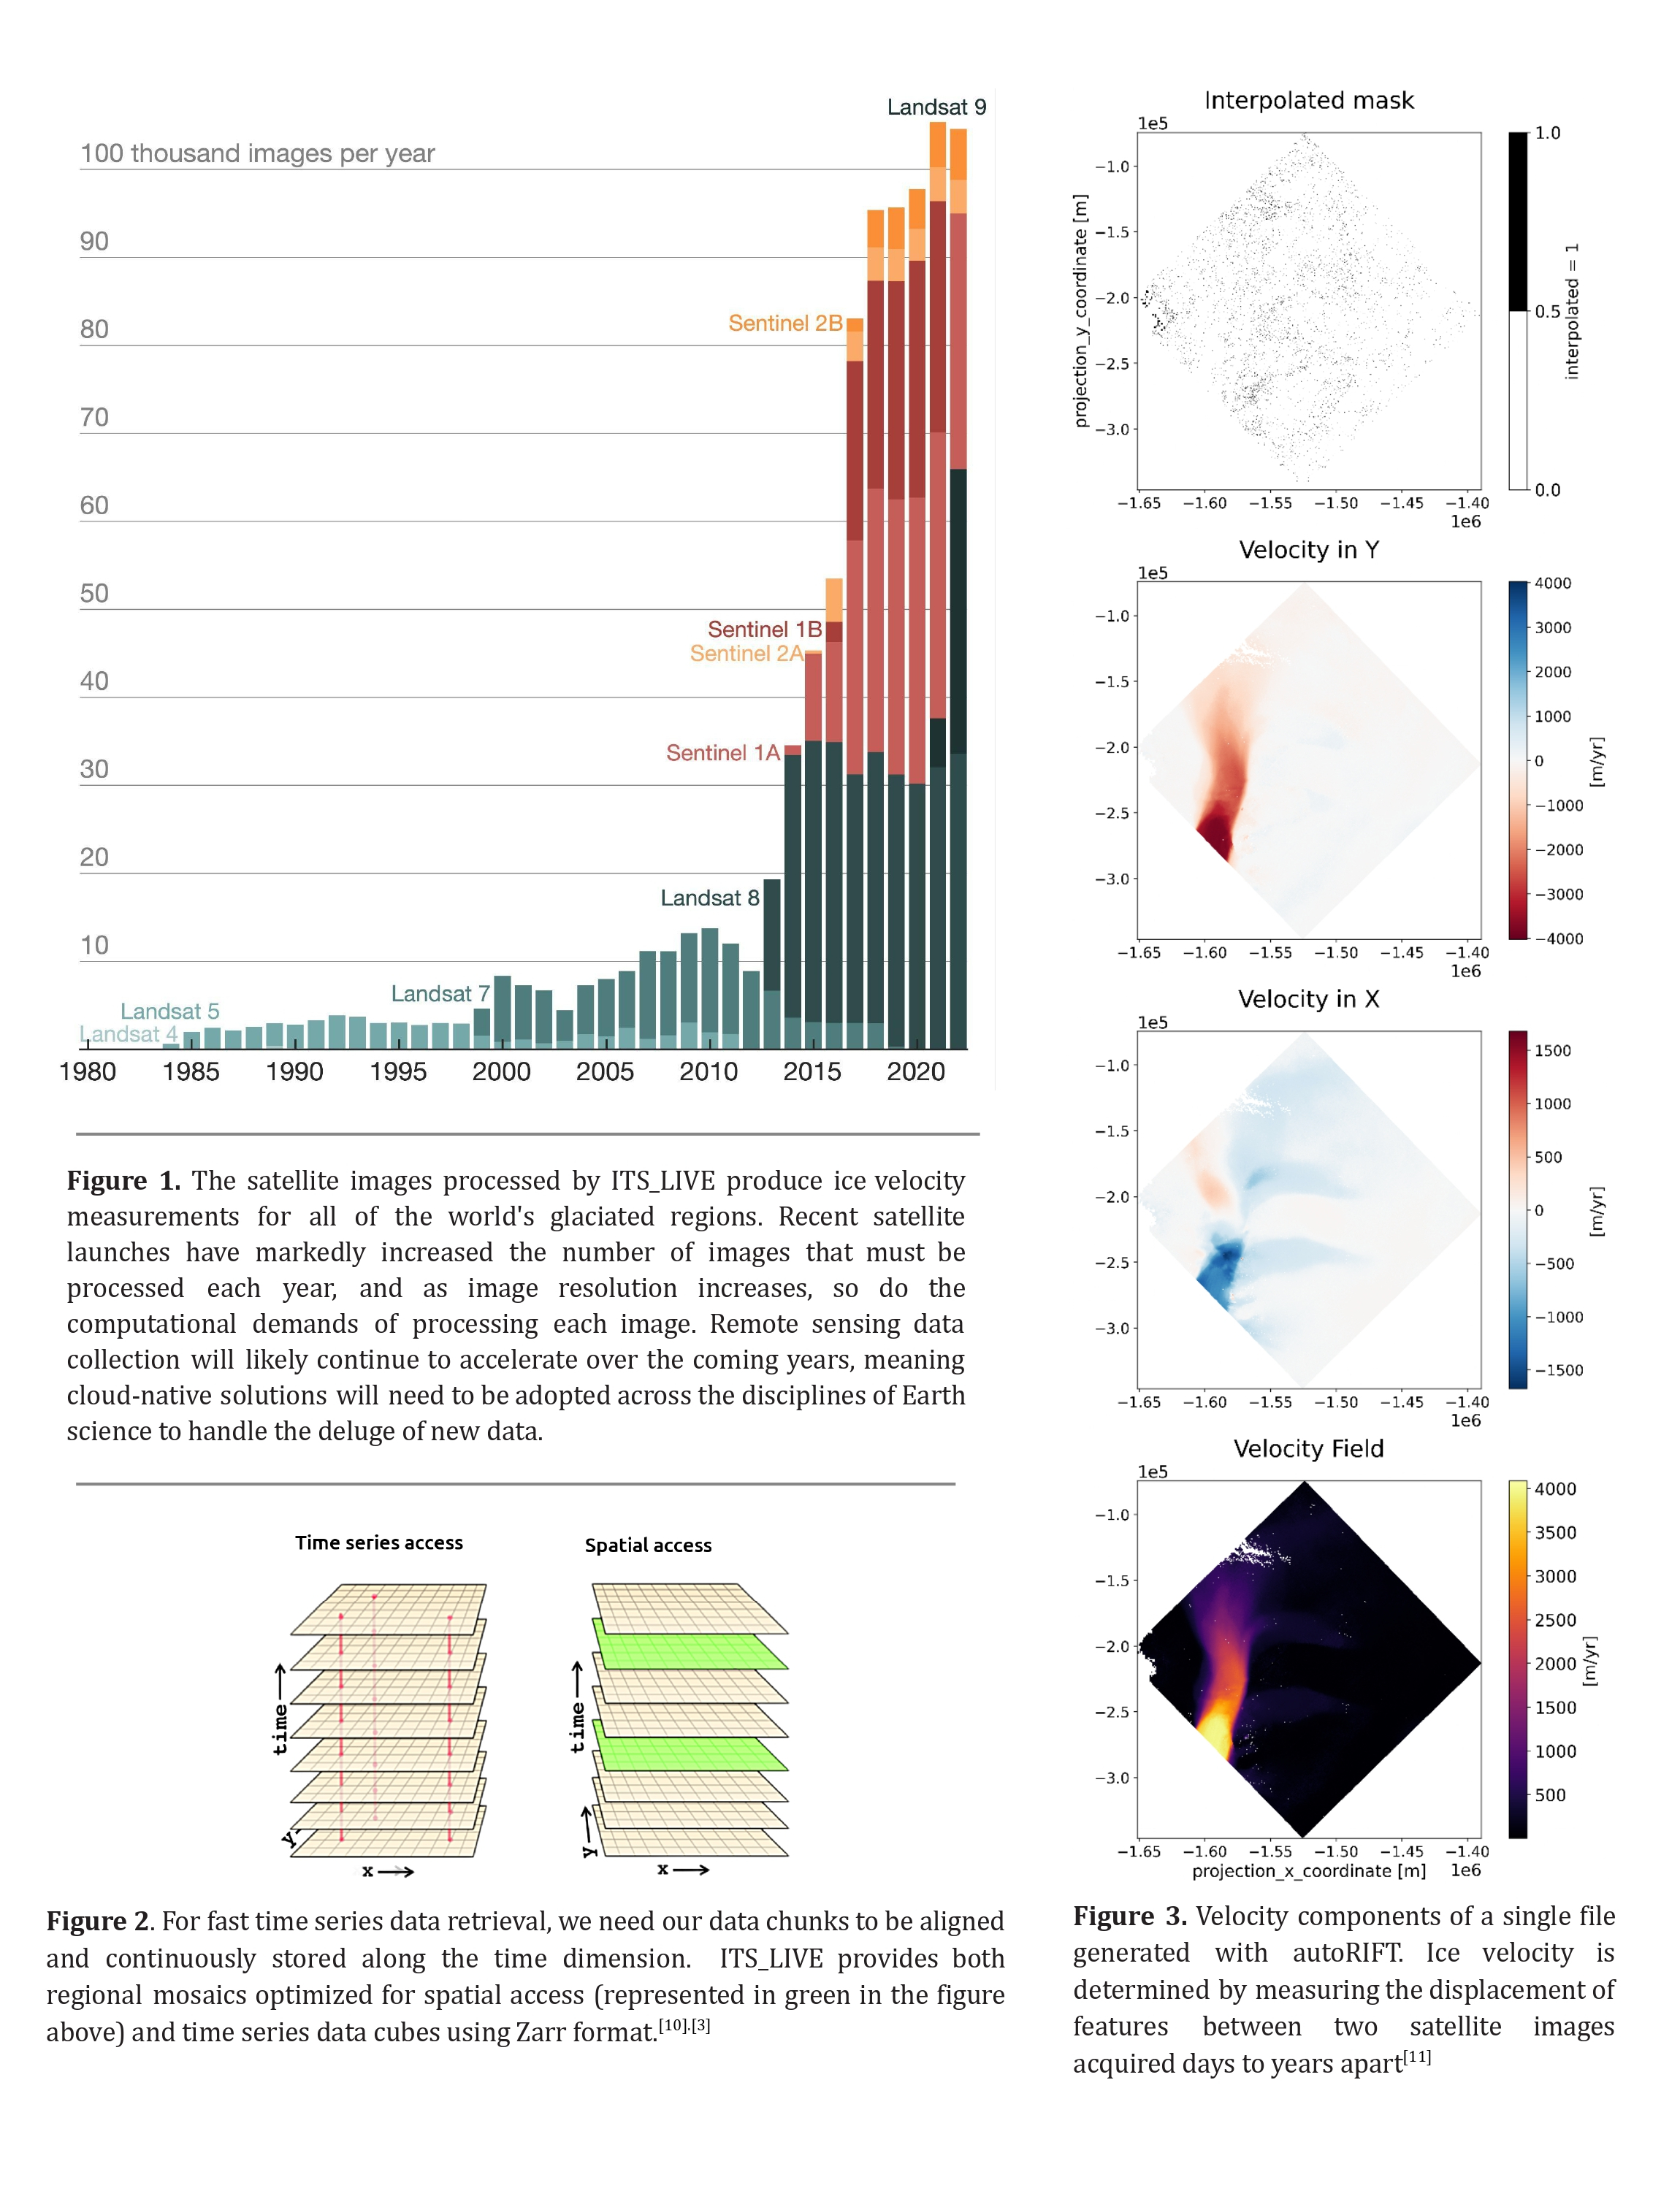
\includegraphics{figures/figure-1-full.jpg}

}

\caption{\label{fig-1}\citep[See][]{Miles2023-yj, Fouilloux2018-jw, Scambos1992-jz}}

\end{figure*}

\begin{figure*}

{\centering 

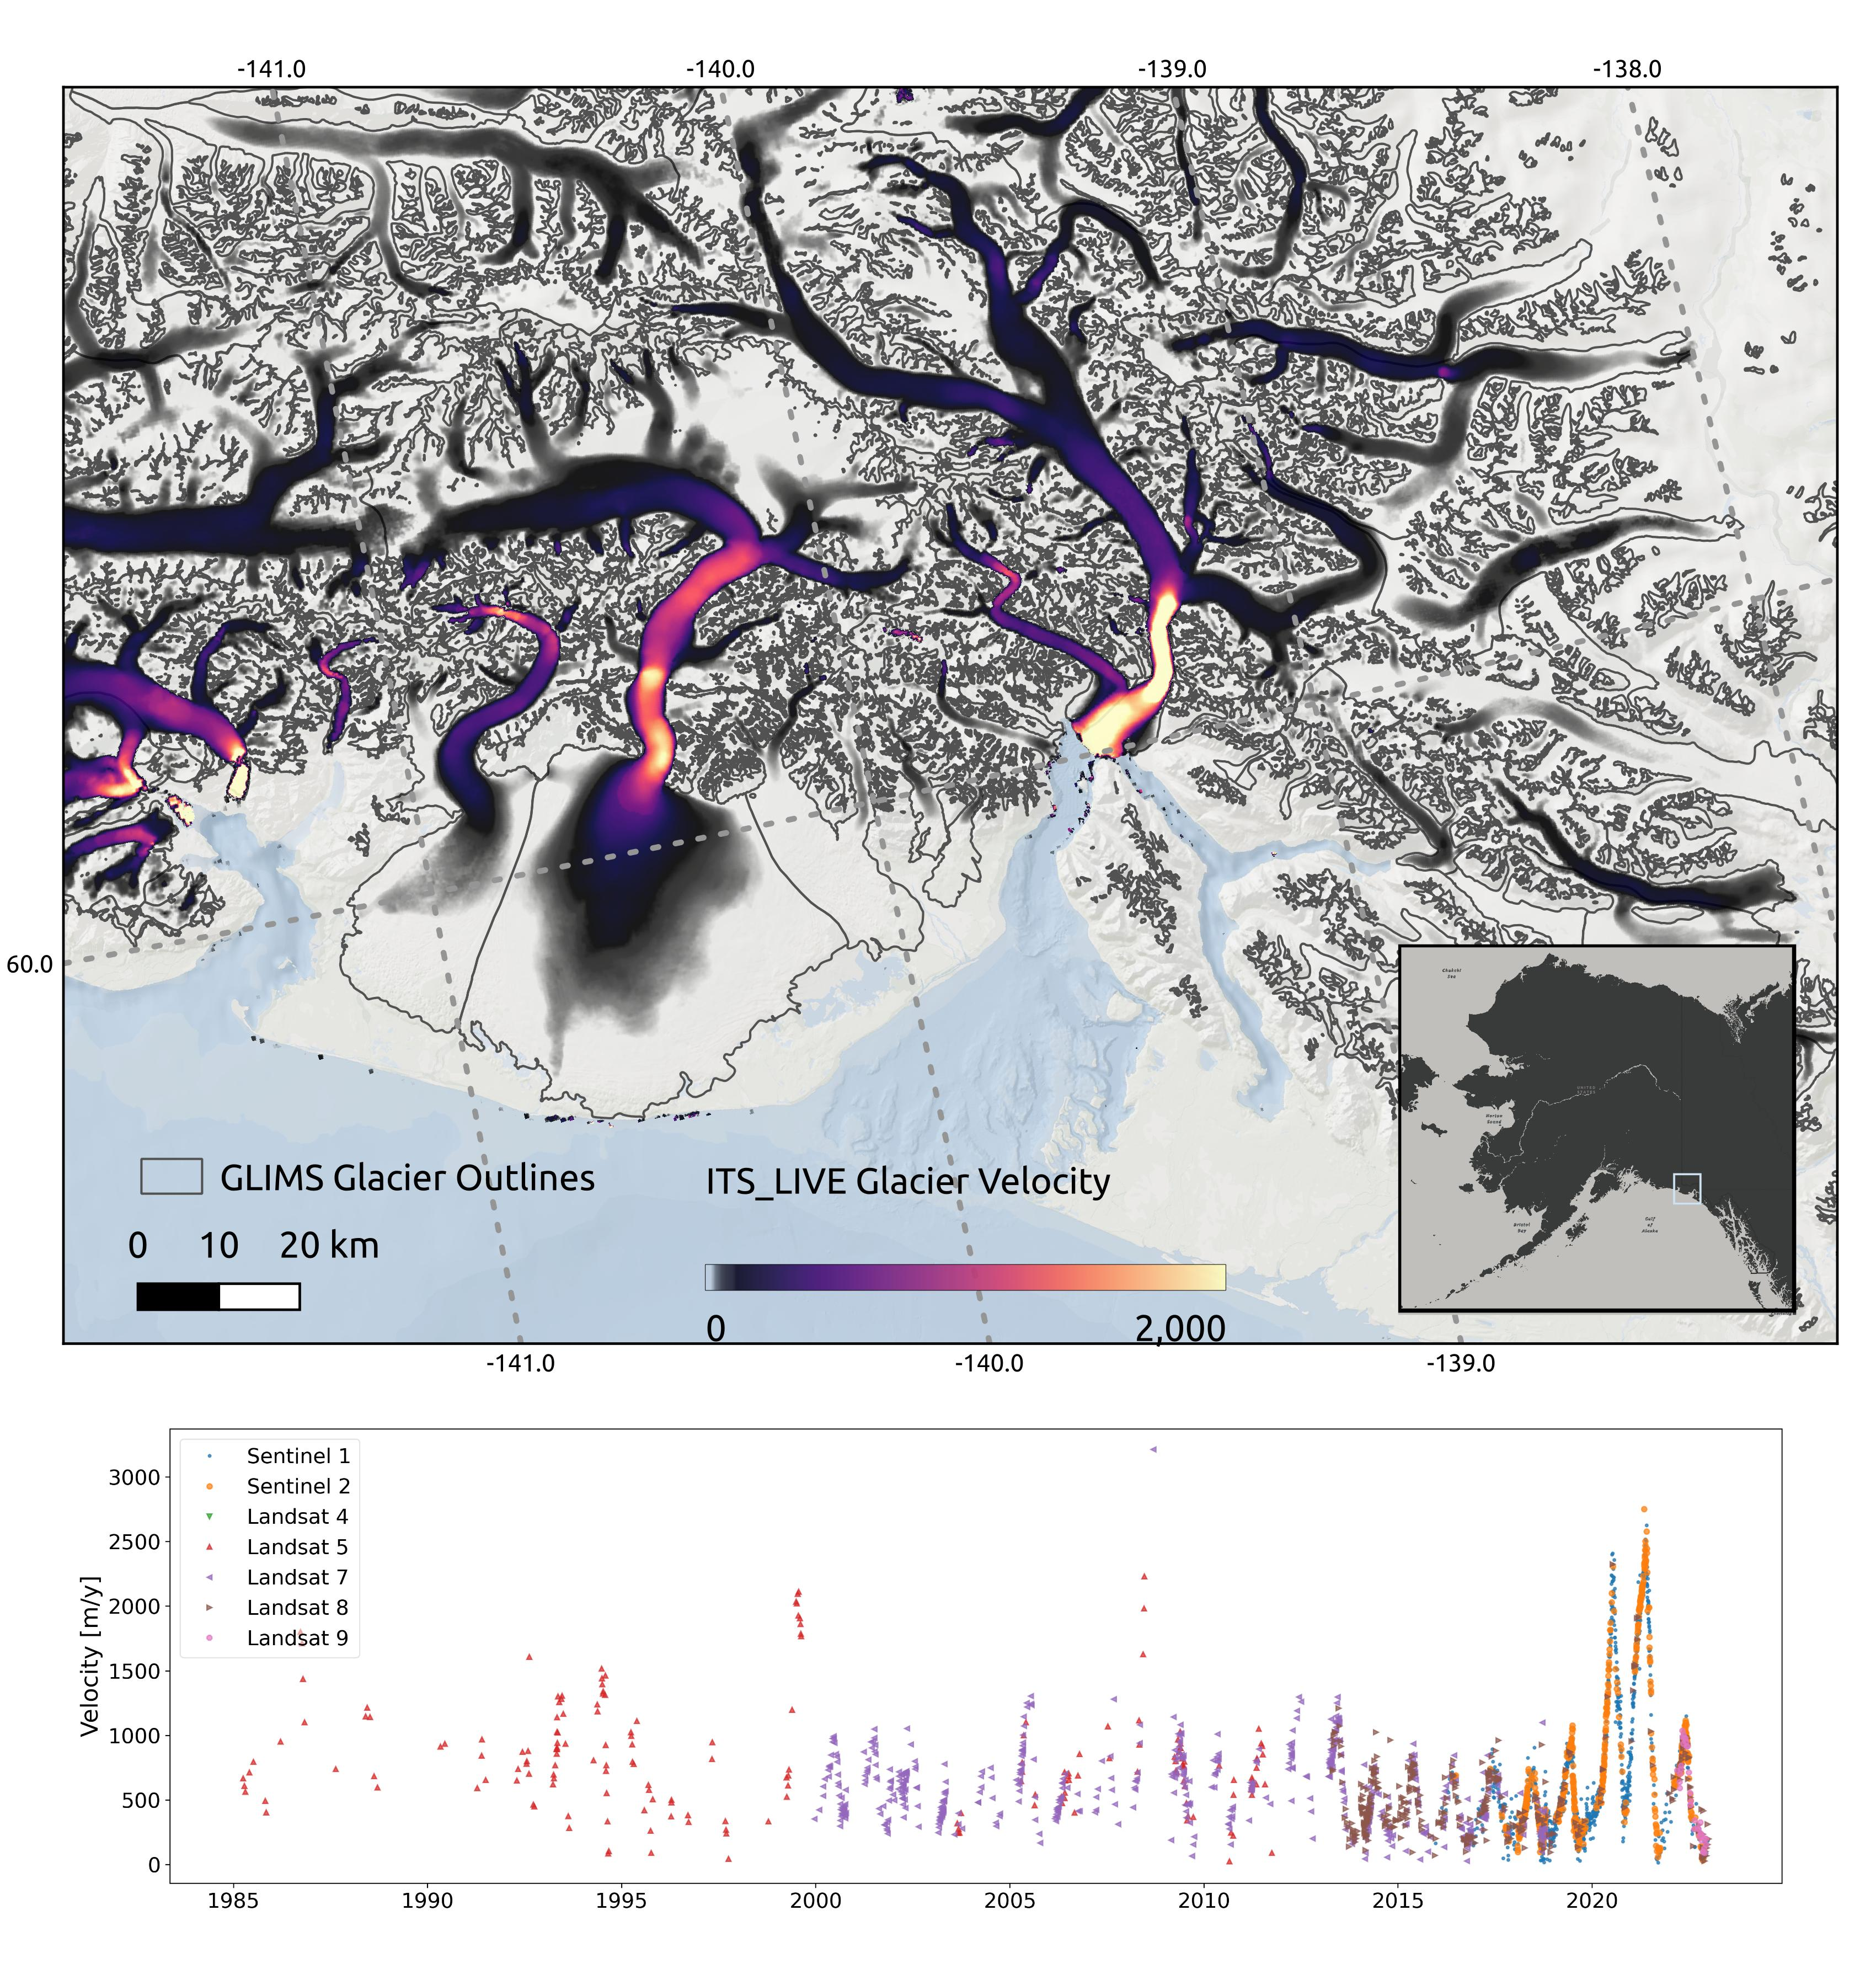
\includegraphics{figures/figure-4.jpg}

}

\caption{\label{fig-2}The Jupyter-based dashboard
https://itslive-dashboard.labs.nsidc.org/ and web based widget
https://nasa-jpl.github.io/itslive-web/ let us query time series of
glacier velocity and export the data into familiar formats like NetCDF
or CSV files. A single time series query can contain more than 200k data
points. Despite the size of the dataset rendering these time series
usually take less than 3 seconds to be completed thanks to the
time-aligned chunking. Malaspina glacier (center) in Alaska is one of
the glaciers that have shown a recent surge in activity (rapid
acceleration). Near real time data processed by ITS\_LIVE has helped
scientists plan field campaigns to place in situ instruments to study
the surge in detail.}

\end{figure*}

\begin{figure*}

{\centering 

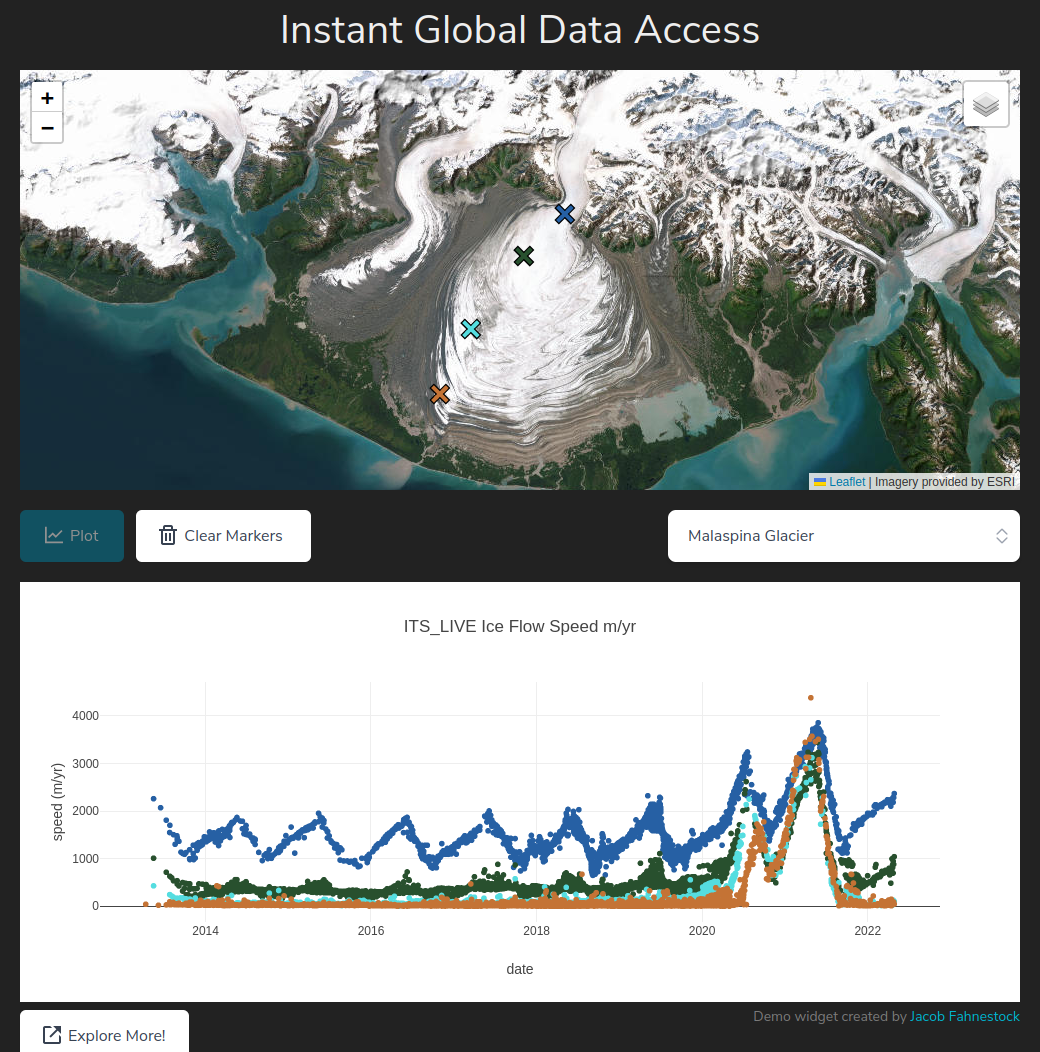
\includegraphics{figures/figure-5.png}

}

\caption{\label{fig-3}ITS\_LIVE gives users who are not familiar with
APIs and programming languages a way to explore the rich dataset and to
begin analysis, regardless of whether they wish to work locally from a
laptop or in the cloud. ITS\_LIVE dashboards allow users to search,
visualize, and download data without the need for a single line of code,
and a client-side only prototype now provides most of the functionality
of the Jupyter-based dashboard but without the need of any back-end
\citep[server][]{Fahnestock2023-fu}}

\end{figure*}

\begin{figure*}

{\centering 

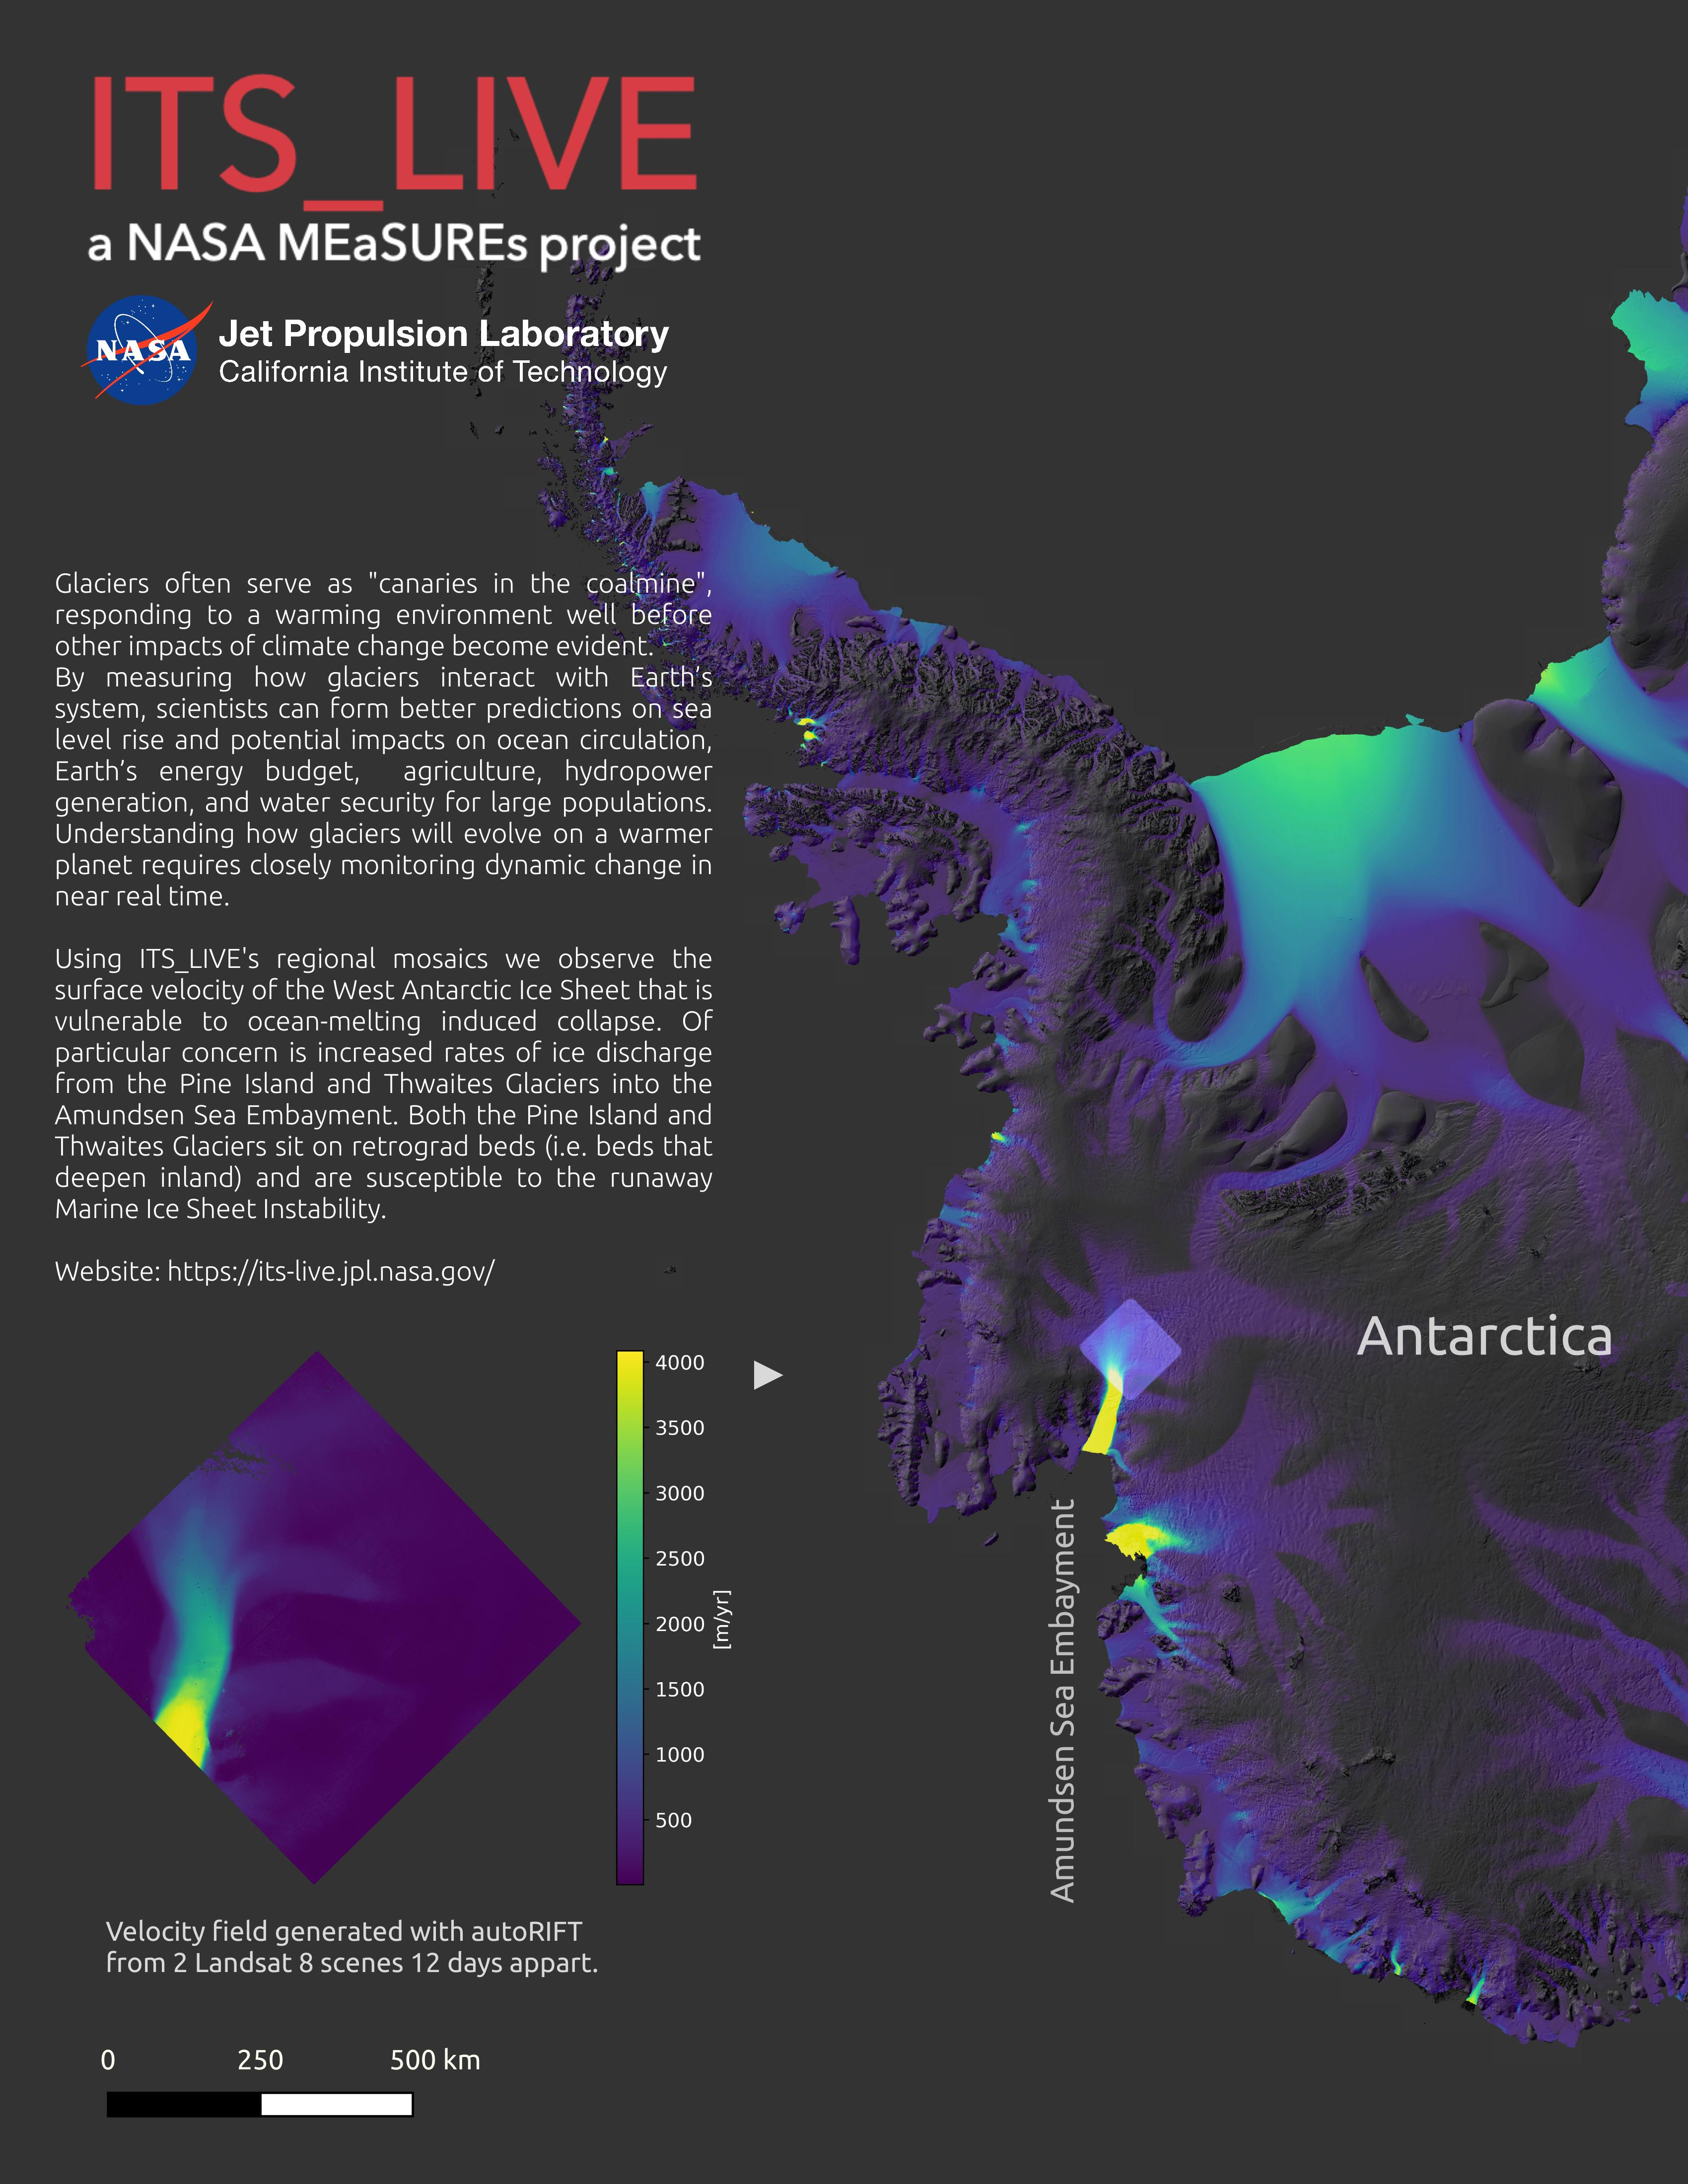
\includegraphics{figures/figure-6.jpg}

}

\caption{\label{fig-4}Info-graphic showing the surface velocity of the
West Antarctic Ice Sheet that is vulnerable to ocean-melting induced
\citep[collapse][]{Joughin2011-mq, Greene2022-uo, Naughten2023}}

\end{figure*}

\begin{figure*}

{\centering 

\includegraphics{figures/figure-7.jpg}

}

\caption{\label{fig-5}What looks like a frequency spectrogram on the
right in this figure is a velocity profile along sampled points in
Malaspina glacier in Alaska (above) , with the first point at the lower
end of the ice (0 km at the left edge). In this plot the ice is flowing
from the right to the left (A to B). One can see the seasonal cycle in
speed (slowest in Fall) in the upper glacier, and the surges of the
Malaspina in indicated years, including 2020 and 2021, when the entire
glacier along this centerline reached speeds \textgreater{} 2500 m/yr,
or 6.8 m/day.}

\end{figure*}

\newpage{}

\textbf{---Keys to success}

Earth Science is undergoing a major transition, from being data-poor to
data-rich. The old paradigm of navigating to a webpage, downloading data
and working with it locally on one's computer is quickly dying. We are
now entering an era where we will expect shared code to link to
low-latency cloud-accessible datasets so the analysis code can run
out-of-the-box and be truly reproducible. By breaking down traditional
disciplinary barriers of engineering, technology, and Earth science,
ITS\_LIVE has developed optimized technical solutions to obstacles that
might otherwise stand in the way of creating, accessing, exploring, and
visualizing such novel and complex datasets. ITS\_LIVE was built on
Findable, Accessible, Interoperable, and Reusable (FAIR) data
principles, and has mitigated many of the challenges surrounding rapid
time series analysis of massive archives. By providing intelligently
structured cloud-optimized glacier velocity data, ITS\_LIVE has reduced
the demand for expertise in remote sensing and geospatial analysis,
making the data more accessible to a broader range of researchers. By
designing to meet user needs and enlisting the help of experts in modern
cloud computing, ITS\_LIVE has built an active and growing community of
scientists that are generating new insights into why and how glaciers
have responded to changes in their environment, giving clues as to what
our future might hold.

\textbf{ACKNOWLEDGMENTS}

The ITS\_LIVE user community for their helpful feedback. Pangeo
community. Copernicus Sentinel data processed by ESA. Landsat data
courtesy of the U.S. Geological Survey. Funding for ITS\_LIVE provided
by the NASA MEaSUREs program.

\textbf{Luis A. López} is a Research Software Engineer currently working
with the National Snow and Ice Data Center in Boulder, Colorado. His
research interests include remote sensing data workflows, cloud
computing and open science. Contact him at luis.lopez@nsidc.org

\textbf{Alex S. Gardner} is the ITS\_LIVE Principle Investigator and a
NASA Research Scientist at the Jet Propulsion Laboratory in Pasadena,
California. He studies the Earth's cryosphere (frozen Earth) with a
particular focus on glaciers and ice sheets and their impacts on sea
level rise and water resources.

\textbf{Chad A. Greene} is a NASA Research Scientist at Jet Propulsion
Laboratory, California Institute of Technology. He uses satellite and
airborne remote sensing to study the Earth's cryosphere, and is a former
editor of the Proceedings of the National Academy of Sciences.

\textbf{Joseph H. Kennedy} is a Computational Scientist at the Alaska
Satellite Facility in Fairbanks, AK. He specializes in building Big Data
processing and analysis platforms for Earth data and studies the Earth
system using HPC models.

\textbf{Maria Liukis} is an Engineering Applications Software Engineer
at the Jet Propulsion Laboratory, Pasadena CA. With a specialization in
scientific programming, she assists scientists in addressing
computational challenges, while also contributing to software
development for various missions and tools.

\textbf{Mark A. Fahnestock} is a Research Professor in the Snow, Ice,
and Permafrost group at the Geophysical Institute of the University of
Alaska Fairbanks. He studies glaciers and ice sheets with a focus on
observational constraints on change


\renewcommand\refname{References}
  \bibliography{bibliography.bib}


\end{document}
